\scanpage{75}
% archive sheet number: 74

\margin{\handwritten{On a un hom (une fois choisi $\bar{k}$ ; d'où une réalisation \deleted{\unsure{$G'|C'$}} de lien $\unsure{\underline{\pi}|\underline{\Pi}}_p(k)$) $\pi_1(k)_K\longrightarrow\unsure{G'|C'}(K)$ d'où un foncteur $(\text{torseurs sous }\pi_1(k)_K)\longrightarrow\text{torseurs sous }G'$ \unsure{Et|et} on prend l'image du torseur sous $\pi_1(k)_K$, défini en interprétant $\pi_1(k)$ comme Galois de l'extension non ramifiée \unsure{universelle} de $K$.}}
pro-fini ``abstrait'' $\handwritten{\pi}_1(k)$, mais on se convainc facilement qu'elles\deleted{\unsure{sont}} sont contenues dans la donnée de ce groupe, $+$ son opération sur la clôture algébrique $\handwritten{\bar{K}}$ de $K$ (ou simplement, sur sa clôture non ramifiée .sur $W$ ...)\handwritten{/}. - Il resterait enfin à déterminer la structure d'effectivité dans la catégorie $\mathrm{Fcriso}(k)$ dé\deleted{\unsure{terminé}}\handwritten{\unsure{terminé}}e par la récette précédente\deleted{\unsure{.} la suggestion naturelle est que $\mathrm{Fcriso}^{\handwritten{+}}(k)$ est engendré par les images de $\mathrm{Fcriso}^{\handwritten{+}}$} Or il est immédiat que l'effectivité d'un \unsure{F-isocrristal|F-isocristal} est invariante par changement de base, en particulier par le changement de base $k\handwritten{\longrightarrow\bar{k}}$, ce qui ramène au cas d'un $k$ algébriquement clos, ou encore au cas de $\underline{F}_p$ . \deleted{En}\handwritten{Dans} \deleted{termes de} la terminologie introduite plus bas, on trouvera donc que les $\unsure{\mathbb{F}|F|E}$-isocristaux effectifs sont ceux qui sont \uline{à pente} $\handwritten{\geq}0$ (i.e. dont toutes les composantes isopentiques \deleted{sont} non nulles sont de pente $\handwritten{>}\ 0$).

\handwritten{8.} Il reste donc à étudier la gerbe $\underline{G}(\underline{F}_p)$, avec s\deleted{\unsure{on}}a \deleted{foncteur fibre} section canonique sur $\underline{Q}_p$, sa structure d'extension, et sa structure d'effectivité.

\margin{\handwritten{\figure{\begin{tikzpicture}\draw (0,0) -- (0.65,0.04) -- (0.65,0.8) -- (1.1,0.8);\end{tikzpicture}}}}
\inserted{\handwritten{8.1.}} Tout d'abord, la donnée du foncteur fibre canonique permet d'identifier $\underline{G}(\underline{F}_p)$ à la gerbe\handwritten{\,}triviale définie par le lien \inserted{\handwritten{$G$}} de cette gerbe. Comme $\mathrm{Fcriso}(F_p)$ avec son foncteur fibre s'identifie à la catégorie des automorphismesde\inserted{$F_E$} vectoriels de dimension finie\inserted{$E$} sur $\underline{Q}_p$, avec le foncteur ``oubli de $F_E$ '', on voit que le lien de la gerbe est l'enveloppe $\underline{Q}_p$-\inserted{pro}algébrique de groupe discret $\underline{Z}$ . Soit $G$ ce groupe affine sur $\underline{Q}_p$ . I\handwritten{l} est évidemment commutatif, donc produit d'un groupe vectoriel $G_u$ par un groupe de t.m. $G_{\deleted{\unsure{m}}r}$ .
\margin{\handwritten{\unsure{réf}\figure{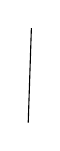
\begin{tikzpicture}\draw (0,0) -- (0.04,1.2);\end{tikzpicture}}}}
Ce dernier est l'enveloppe \inserted{de type} multiplicati\deleted{ve}\handwritten{f} du groupe $\underline{Z}$, et il s'ensuit aussitôt que c'est le groupe de t.m. dont le groupe des caractères sur $\handwritten{\bar{\underline{Q}}}_p$ est donné par
\[
\handwritten{\Gamma}=\handwritten{\bar{\underline{Q}}}_p^{\handwritten{*}}\ ,
\]
\handwritten{(}isomorphisme compatible avec l'action de $\operatorname{Gal}(\handwritten{\bar{\underline{Q}}}_p/\underline{Q}_p)$ ). D'autre
